\documentclass[journal]{vgtc}                % final (journal style)
%\documentclass[review,journal]{vgtc}         % review (journal style)
%\documentclass[widereview]{vgtc}             % wide-spaced review
%\documentclass[preprint,journal]{vgtc}       % preprint (journal style)
%\documentclass[electronic,journal]{vgtc}     % electronic version, journal

%% Uncomment one of the lines above depending on where your paper is
%% in the conference process. ``review'' and ``widereview'' are for review
%% submission, ``preprint'' is for pre-publication, and the final version
%% doesn't use a specific qualifier. Further, ``electronic'' includes
%% hyperreferences for more convenient online viewing.

%% Please use one of the ``review'' options in combination with the
%% assigned online id (see below) ONLY if your paper uses a double blind
%% review process. Some conferences, like IEEE Vis and InfoVis, have NOT
%% in the past.

%% Please note that the use of figures other than the optional teaser is not permitted on the first page
%% of the journal version.  Figures should begin on the second page and be
%% in CMYK or Grey scale format, otherwise, color shifting may occur
%% during the printing process.  Papers submitted with figures other than the optional teaser on the
%% first page will be refused.

%% These three lines bring in essential packages: ``mathptmx'' for Type 1
%% typefaces, ``graphicx'' for inclusion of EPS figures. and ``times''
%% for proper handling of the times font family.

\usepackage{fancyhdr}
\usepackage{float}
\usepackage{mathptmx}
\usepackage{graphicx}
\usepackage{times}
\usepackage{balance}
\usepackage[nooneline,hang,it,IT]{subfigure}
\usepackage{lastpage}

%% We encourage the use of mathptmx for consistent usage of times font
%% throughout the proceedings. However, if you encounter conflicts
%% with other math-related packages, you may want to disable it.

%% This turns references into clickable hyperlinks.
\usepackage[bookmarks,backref=true,linkcolor=black]{hyperref} %,colorlinks
\hypersetup{
  pdfauthor = {},
  pdftitle = {},
  pdfsubject = {},
  pdfkeywords = {},
  colorlinks=true,
  linkcolor= black,
  citecolor= black,
  pageanchor=true,
  urlcolor = black,
  plainpages = false,
  linktocpage
}

%% If you are submitting a paper to a conference for review with a double
%% blind reviewing process, please replace the value ``0'' below with your
%% OnlineID. Otherwise, you may safely leave it at ``0''.
\onlineid{0}

%% declare the category of your paper, only shown in review mode
\vgtccategory{Research}

%% allow for this line if you want the electronic option to work properly
\vgtcinsertpkg

%% In preprint mode you may define your own headline.
%\preprinttext{To appear in an IEEE VGTC sponsored conference.}

%% Paper title.

\title{AiPoker - An Implementation of a Poker Agent}

%% This is how authors are specified in the journal style

%% indicate IEEE Member or Student Member in form indicated below
\author{John Holl\'en, Robin Berntsson, Simon Bergstr\"om}
\authorfooter{
%% insert punctuation at end of each item
\item
 Simon Bergstr\"om, Media Technology student at Link\"oping University, Sweden, e-mail: simbe109@student.liu.se.
\item
  Robin Berntsson, Media Technology student at Link\"oping University, Sweden, e-mail: robbe482@student.liu.se.
\item
  John Holl\'en, Media Technology student at Link\"oping University, Sweden, e-mail: johho982@student.liu.se.
}

%% Abstract section.
\abstract{ 
Poker is a well known card game worldwide and has become very popular to play online for the past few years. This project aims at investigating the possibilities with creating a Poker Agent using the logic of a Monte Carlo Tree Search in combination with a few smaller well known algorithms. The result is a poker agent which plays with realistic reasoning.
}
%% Keywords that describe your work. Will show as 'Index Terms' in journal
%% please capitalize first letter and insert punctuation after last keyword
\keywords{Monte Carlo Tree Search, Texas Hold'em}



%%%%%%%%%%%%%%%%%%%%%%%%%%%%%%%%%%%%%%%%%%%%%%%%%%%%%%%%%%%%%%%%
%%%%%%%%%%%%%%%%%%%%%% START OF THE PAPER %%%%%%%%%%%%%%%%%%%%%%
%%%%%%%%%%%%%%%%%%%%%%%%%%%%%%%%%%%%%%%%%%%%%%%%%%%%%%%%%%%%%%%%%

\begin{document}

\fancypagestyle{empty}{
 \fancyhf{}
 \fancyhead[R]{TNM095 \\* HT1 2014}
 \fancyhead[C]{Artificial Intelligence for Interactive Media}
}

\pagestyle{fancy}
\rhead{TNM095 \\* HT1 2014}
\chead{Artificial Intelligence for Interactive Media}
\lhead{\empty}
\cfoot{\empty}
\rfoot{Page \ \thepage \ of \ \pageref{LastPage}}
\pagenumbering{arabic}
%% The ``\maketitle'' command must be the first command after the
%% ``\begin{document}'' command. It prepares and prints the title block.

%% the only exception to this rule is the \firstsection command
\firstsection{Background}
\maketitle 
Texas Hold'em is a popular variant of poker, not just to play with friends but also online against other people for money. The challenge of creating the best poker agent has attracted a lot of people and is a popular subject in AI development.
\\*\\*
\textbf{Type of Games}\\*
There are many different types of games and the strategy to solve these games depends on the type of game. In game theory games can be classified due to the knowledge of the transition to a new state within the game depends on a stochastic process, and if there is hidden information. Poker belongs to the most difficult kind of games to solve discretely since it is an stochastic game with imperfect information\cite{Kleij}.
\\*\\*
\textbf{Perfect Information vs Imperfect Information}\\*
In perfect information games both players can observe the complete state of the game at any given time, this is the case in games such as Chess and Go. Contrary to this we have imperfect information games where each player is unable to observe the complete state, one example of this is poker were neither player can see the other player's cards. 
\\*\\*
\textbf{Deterministic vs Stochastic}\\*
In deterministic games the next state of the game is uniquely determined by an action taken at the current state. In contrast, a stochastic game is a game where the player does not have control over the transition to the next state. For example in poker where the new cards are drawn from a scrambled deck.  

\begin{table}[h]
\begin{tabular}{|l|l|l|}
\hline
              & Perfect Information  & Imperfect Information \\ \hline
Deterministic & Chess, Go            & Battleships           \\ \hline
Stochastic    & Backgammon, Monopoly & Poker                 \\ \hline
\end{tabular}
\caption{\label{tab:table1} Table showing different categories of games.}
\end{table}

The classification in Table.\ref{tab:table1} shows that games like Chess and Go belong to the category of games that are less complex to solve with an AI agent. Poker belongs to one of the most complex games to solve, since it is both stochastic and has imperfect information.

\subsection{Related Work}
\subsubsection{Game Theory}
In 1997 Koller and Pfeffer\cite{Koller} made a program called Gala. Gala uses strategies from game theory to find optimal strategies in imperfect information games. With the help of Gala they were able to solve several games but they came to the conclusion that the number of states in poker is too large to be solvable with the hardware available at the time. However, they suggested that maybe it was possible to map several similar states onto one abstract state resulting in an abstract game tree much smaller than the original. 
It was from this idea that (Billings et al 2003)\cite{billingsburch} successfully abstracted the game down from a search space of $O(10^{18})$ to $O(10^{7})$. They then used Linear optimization to find a Nash equilibrium solution to the game. From this they could take any action, map it to the abstract game tree, find a solution and then map it back to the real game. This resulted in a poker agent (PsOPti) that was far better than anything else at the time. 

\subsubsection{Expert Systems}
Billings et al.(1998)\cite{billingspapp} developed an AI agent called Loki. It is an expert system that uses a set of rules and formulas based on the strength of the cards to determine the next action. It uses no opponent modeling in two player poker. It can be challenging to define strong expert systems as it can be hard to define rules that cover all aspects of the game. There can also be problems with conflicting rules and missing rules (situations that are not covered by any rules). Another problem is that expert systems require that you have great knowledge about the game as the AI will never play better than the defined the rules.

\subsubsection{Opponent Modeling}
Papp (1998)\cite{papp} was the first to try to extend Loki with opponent modeling. The opponent model was quite simple and just counted the opponents actions in the different game stages (preflop, flop, turn, river). This simple model increased the strength of the AI.  

Davidson et al. (2000)\cite{davidson} tried to improve the opponent modeling in Loki with artificial neural networks (ANNs) to predict the opponent's actions, and achieved about 85\% accuracy when predicting the moves. This is a significant improvement over the previous implementation, and the new system was named Poki. The problems with ANNs is that they can be slow to train, thus they will play weakly against players who frequently change their style of playing.

\subsubsection{Search Trees}
Billings et al. (2004)\cite{billingsdavidson} were some of the first to use game tree search in a poker AI. Their AI, Vexbot uses two modified versions of Expectiminimax called Miximax and Miximix that extends Expectiminimax to games with hidden information. Vexbot makes an exhaustive depth first search of the entire search tree for a two player game of poker. 

Van den Broeck et al. (2009)\cite{broeck} were the first to apply Monte Carlo tree search for poker agents. They focused on 10 player no-limit poker. 10 player no-limit poker has enormous game trees which make methods such as Miximax and Miximix impossible to use. Since it is impossible to search the whole game tree, sampling parts of the game tree is the only option. 

\subsection{Monte Carlo Methods}
Monte Carlo methods is a class of algorithms that rely on random sampling to obtain a numerical estimate of a complex problem. The method was invented by Stanislaw Ulam while working with the nuclear weapon program at Los Alamos in the 1940s \cite{Metropolis}. 
\begin{figure}[here]
  \begin{center}
    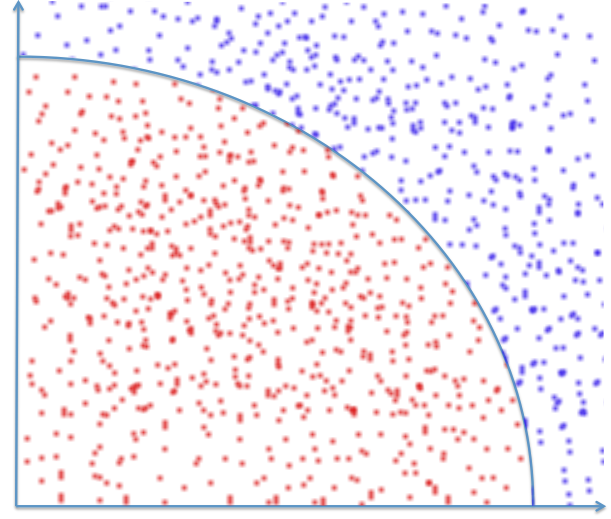
\includegraphics[scale=0.35]{img/integralexample.png}
    \caption{\label{fig:integralex} An illustration of how to determine the value of an integral with the help of Monte Carlo methods.}
  \end{center}
\end{figure}
 
One possible use for Monte Carlo methods is to determine the value of an integral as illustrated in Fig.\ref{fig:integralex}. By randomly placing dots and labelling them as either under or over the function value an estimate of the area can be achieved. By taking the area of the square encapsulating the function times the ratio between the number of points under the function and the total amount of points. The approximated value given by a Monte Carlo method will converge to the correct value as the number of sample points goes to infinity\cite{Kleij}.

The insight that random sampling can be used to solve problems that are too complex to solve analytically can be used to evaluate the best action in huge game trees. For a given node $N$, the value can be estimated by running a number of simulations of how the game may end from that node. The result from those simulations can then be used to give an approximation for the value of that node. As the number of nodes grows it will converge to the result from a Minimax search. 

Monte Carlo tree search (MCTS) has made huge improvements for games that were previously very hard for AIs. One example is Go in which agents powered by MCTS now can compete with the best players in the world.

\section{Theory}
\textit{(If you already are familiar with the game of Texas Hold'em, you can skip to section 2.2).}
\subsection{Texas Hold'em no Limit}
There are many forms of poker, the most popular being Texas Hold'em. Texas Hold'em can be played in two different ways, limited and no-limit. In limited poker the bet and raise amount are fixed, there is also an upper limit of how many times the players raise. However in no-limit poker there is no limit for how much the players can bet, and there is also no limit for how many times the payers can raise.
\subsubsection{Main Concept}
The aim of the game is to win as much money as possible. When a player is out of money, that player has lost. When everyone except one player has run out of money the game is over and a winner is designated.

Every round each player gets two cards on hand, and five cards are dealt to the table. The player with the best combination of these seven cards wins the round. 

In order to make sure for every round that there is money in the pot, there is small entry fee called the blind. The blind also takes away the risk of players being too defensive. 
The blind consists of two amounts called the big and the small blind. When the game starts a player gets randomly selected to pay the big blind and the player to the left of him/her gets to pay the small blind. When a new round begins, the blinds move one step to the left. If there are only two players they just switch big and small blind every round. The big blind is the double amount of the small blind and is a pre set sum.

The game consists of five stages where the players can decide how to proceed in the game.
The stages are called:  pre-flop, flop, turn, river and showdown.

\subsubsection{The Game Stages}

\textbf{Pre Flop}\\*
In this stage the players get two cards each from the dealer. These cards are called the pocket cards and after the cards have been dealt, the first betting round begins. If a player bets or raises all other players get the opportunity to either call, raise or fold max three times, after that the players who have not folded move on to the flop.
\\*\\*
\textbf{Flop}\\*
The flop is when the dealer deals the three first cards on the table. These cards are visible to all players. The pocket cards can now be combined with the flop cards in order to create a full hand. The players will make moves in the same procedure as in the pre-flop stage.
\\*\\*
\textbf{Turn}\\*
Now the dealer adds a fourth card to the table. The players will now bet again.
\\*\\*
\textbf{River}\\*
The dealer adds a fifth card to the table. This is the last card which is dealt. After the last betting round, the game moves on to showdown. 
\\*\\*
\textbf{Showdown}\\*
In this phase the final betting is completed and the players who have not folded yet will now show their cards in order to decide who is the winner of this round. The winner will get the full pot and then a new round will start with the pre flop.
\\*\\*
\textbf{The different five combination of cards}\\*
There are nine different types of combination of cards and here they are listed in descending order:
\begin{itemize}
  \item \textit{Straight Flush}: When the player has five cards in a consecutive order of value within the same suit. If more than one player have a Straight Flush the player with the highest values of his/her cards wins. The best variant is the Royal Straight Flush when the player has Ace, King, Queen, Jack and a ten within the same suit.
  \item \textit{Four of a kind}: It is a hand that contains four of the same value in all the different suits. If more players have the same type of hand the hand with the highest four of a kind wins.
  \item \textit{Full House}: This hand is a combination of three of a kind and a pair. If more than one player have a Full House the player with the highest three of a kind wins. If more players have the same three of a kind, the player with the highest pair wins.
  \item \textit{Flush}: A flush is when a player has five cards within the same suit, if more than one player have a flush the one with the highest card wins. If they have the same highest card then the the second highest card is checked and so on.
  \item \textit{Straight}: When you have five cards in a consecutive order of value in different suits. If more than one player has a Straight then the player with the highest card wins.
  \item \textit{Three of a Kind}: When you have three cards of the same value, if more than one player has a Three of a kind then the player with the highest value of the cards wins.
  \item \textit{Two Pair}: When a player has two pair of cards, if more than one player have a two pair the player with the highest pair has the best hand between them.
  \item \textit{One Pair}: When you have one pair of cards, if more than one player have a one pair the player with the highest pair has the best hand between them.
  \item \textit{High Card}: If the card does not match any of the types above then the card with the highest value is considered. 
\end{itemize}

These rules are the most basic rules and some special cases exists that is not described above, for a more detailed guide of the rules visit : \cite{pokerstars}

\subsection{Characteristics of a Poker Player}
Like previously described poker is a stochastic game. That makes it hard to define what a good poker player is. A good poker player does not always have to be the one who is playing optimally. Some of the main characteristics of a good poker player is that he/she can read his/her opponents strategy or way of playing, has knowledge about when having a good hand to play and know when to play that hand\cite{pokerlistings}.

A player who tries to maximize his/her winnings will have to use bluffing. This applies to both of the cases when the player holds good cards, and when the player holds bad cards. If a player never bluffs his or her strategy becomes predictable and it becomes obvious that the player has good cards as soon as he or she bets. This will lead to the opponent folding and the size of the winning pot being small. 
In the second case, the player might have bad cards. If the player uses bluffing it is possible for him/her to win games where the opponent has better cards.  

\subsection{Game Trees and the Motivation for Monte-Carlo Tree Search}
A game tree is a tree structure that from a given state in the game describes all moves to all possible endings of the game.
\begin{figure}[here]
  \begin{center}
    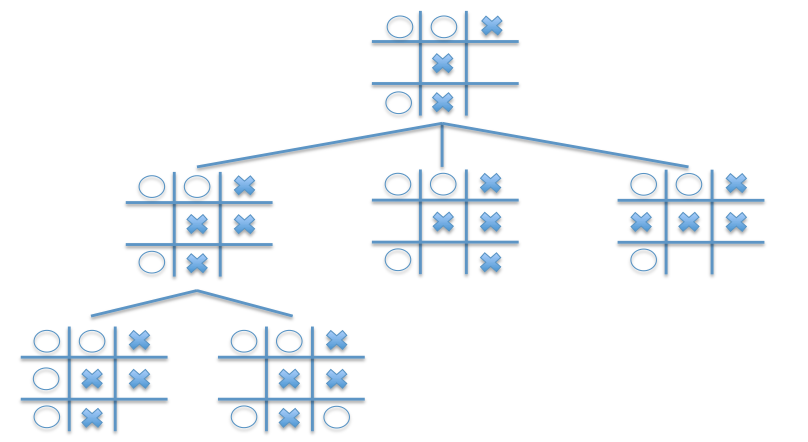
\includegraphics[scale=0.30]{img/MiniMaxGameTree.png}
    \caption{\label{fig:gametree} Part of a tic-tac-toe game tree.}
  \end{center}
\end{figure}

The above example shows a part of a tic-tac-toe game tree. Every node represents a possible state in the game with the root node being the current state and every edge is the action leading to that state. 
The size for a game tree grows very fast when the possible actions that can be taken in each state increase. For example the game tree for an empty tic-tac-toe board has $255168$ leaf nodes. Two player Texas Hold'em has a search space size of $O(10^{18})$\cite{billingsdavidson}.

With the help of game trees computers can reason about the consequences of their actions and many of the most used AI algorithms are based on them. One of the most used tree search algorithms is the Minimax algorithm. Minimax assumes that both players play an optimal strategy. This means that the player who tries to find the best move always selects the actions that will give that player the highest reward thus these nodes are call MAX-nodes. On the other hand the opponent will always select the actions that will give the player the lowest reward and these nodes are called MIN-nodes. The value for each leaf node is determined by a heuristic and the value is back propagated up the tree depending on the parent node. Minimax will search the game tree depth first and the result will be the action which gives the highest reward. 

Expectiminimax is the continuation of the Minimax algorithm that allows for stochastic events in the game tree such as drawing cards in a game of poker. Expectiminimax trees add an additional type of nodes, chance nodes. At chance nodes a child $c$ is chosen with some probability $P(c)$. This means that a chance node for drawing a card from a deck of cards has $52$ children with a uniform probability distribution of $1/52$. The value for a chance node is the weighted average of all its children\cite{Kleij}.

The problem with Minimax and Expectiminimax is that they use depth first search, this poses a problem for games such as poker which have such a big game tree that it can not be fully searched in a reasonable amount of time.

It was this problem that led to the development of Monte Carlo tree search (MCTS). Monte Carlo tree search works around the need to search the game tree exhaustively by estimating the best action by sampling the tree in its most promising parts.  

\section{Method}
\subsection{Basic Game Engine}
In order to even begin implementing an AI, the core poker game had to be implemented first. This was made by first implementing an agent that played at random. For simplicity the game implemented in this study is a two player game with the limited edition of Texas Hold'em where a human player faces a computer AI. 

\subsection{AI-techniques}
A couple of different AI-techniques were implemented in this study. They are described in this section. Also some tests where the different AIs compete against each other were made. The results from these tests are presented in the Result section.

\subsubsection{Monte Carlo Tree Search}
MCTS is a best-first search strategy. Every node $N$ in the tree contains two values, an estimate of the expected reward $v_{i}$ and the number of times the node has been visited $n_{i}$. MCTS only starts with the root node and incrementally builds the tree by repeating the following 4 steps:\\*\\*
\textbf{Selection}
\\*Selection is made by starting from the root node and then recursively select nodes until a leaf node is reached (this does not have to be a leaf of the game tree). To determine which node is the optimal one, the upper confidence bounds formula Eq.\ref{eq:upperconfidence} is used \cite{levente}. 

\begin{equation} \label{eq:upperconfidence}
	v_{i} + C \cdot \sqrt{\frac{\ln (N)}{n_{i}}}
\end{equation}
The first term $v_{i}$ is the estimated reward of the node and is responsible for exploitation of good nodes, the second term is made up by the total number of visits of the parent node $N$ and the total number of visits of the current node $n_{i}$. The constant $C$ allows tuning of the exploration-exploitation trade-off. 
\\*\\*
\textbf{Expansion}
\\*If the leaf node reached is not a terminating node, which means that the game is not over at the current node. Then create one or more child nodes from the node currently at. This step is illustrated in Fig.\ref{fig:expansion}.
\begin{figure}[here]
  \begin{center}
    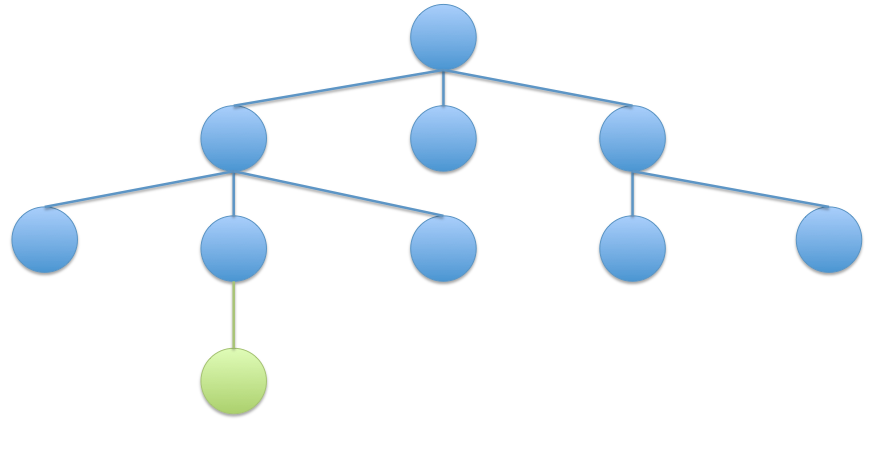
\includegraphics[scale=0.28]{img/tree1.png}
    \caption{\label{fig:expansion} Illustration of how the green node is added to the tree.}
  \end{center}
\end{figure}
\\*\\*
\textbf{Simulation}
\\*The third step in MCTS is the simulation step. Here a game is simulated from the state in the new node until the game has ended. The value of the reached result (won amount of money) is recorded.
\\*\\*
\textbf{Backpropagation}
\\*The last step is to update the expected value and the number of times visited for all nodes along the explored path by backpropagating the recorded result from the simulation step. This step is illustrated in Fig.\ref{fig:backprop}.
\begin{figure}[here]
  \begin{center}
    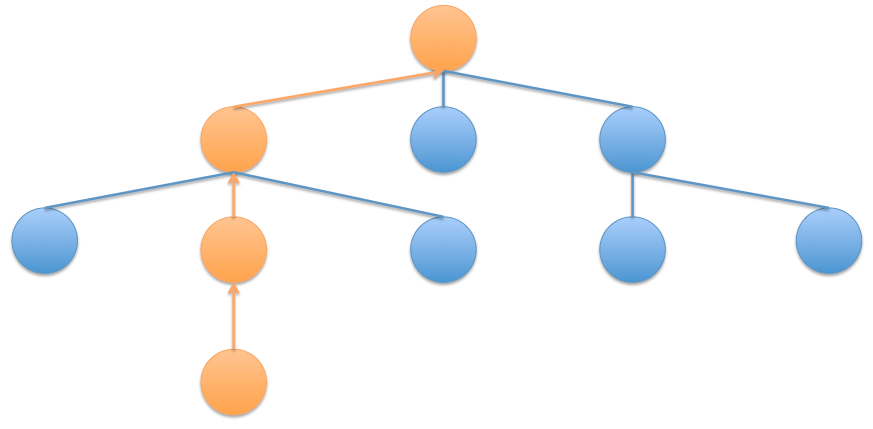
\includegraphics[scale=0.28]{img/tree2.png}
    \caption{\label{fig:backprop} Illustration of how the path to the node is updated with the score from the simulation in the whole tree.}
  \end{center}
\end{figure}
When the back propagation has been done the whole chain starts over again starting with the selection stage\cite{Chaslot}. The use of the upper bounds confidence selection method makes the game tree grow asymmetrically as it focuses its search in the more promising parts of the tree.

One of the advantages of MCTS is that it can be interrupted at any time but still give a valid result. However the quality of the result will increase the longer time MCTS keeps running.

\subsubsection{Hand Strength}
MCTS simulates a set of outcomes in a game to calculate what action to make but it does not consider the strength of the cards on hand. To add this logic to the agent the Hand Strength algorithm was implemented. Hand Strength returns a probability of how strong the current cards on hand are together with the cards on the table, compared to all possible cards that the opponent might have on hand. This probability of the Hand Strength may, at the earliest be calculated when the flop has been dealt\cite{wenkai}.

The Hand Strength is calculated by comparing the cards on the hand with all possible combinations of two cards that the opponent can have and sum the times the agent's cards wins compared to the opponent and divide by the number of combinations that was simulated.

\subsubsection{Hand Potential}
The hand potential algorithm calculates the strength of the cards on hand as the game goes on. The algorithm is similar to the hand strength algorithm. The difference is that the Hand Potential algorithm considers all possible cards that have not been revealed yet. It is also heavier to calculate since it has to go through every possible combination of cards that could possibly end up on the table whereas the Hand Strength algorithm only looks at the revealed cards. It also takes into account every possible card the opponent might have on hand\cite{wenkai}.

\subsubsection{Effective Hand Strength}
By combining the hand strength with the hand potential a probability of winning can be calculated. This is called the effective hand strength and is calculated as follows\cite{wenkai}:

\begin{equation} \label{EHS}
	EHS = HS \cdot (1-NPot) \cdot PPot
\end{equation}
Where $HS$ is the value obtained from the Hand Strength algorithm, $NPot$ is the negative potential from the Hand Potential and $PPot$ is the positive potential from the Hand Potential.

\subsubsection{Bucketing}
Since effective hand strength (EHS) needs at least the flop to be revealed in order to be used for decision making, the Bucketing algorithm was implemented  as a complement to the EHS algorithm. This algorithm is only used in in the pre-flop phase where no cards are visible on the table \cite{schweizer}.
\begin{figure}[here]
  \begin{center}
    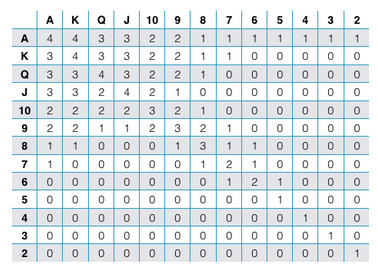
\includegraphics[scale=0.60]{img/bucketlist.png}
    \caption{\label{fig:bucketlist} The bucket list.}
  \end{center}
\end{figure}
\\*The table in Fig.\ref{fig:bucketlist} gives every two card combination a value between 0 and 4 where 4 is a good combination and 0 is a bad combination. This list is the source of decision making in the pre-flop phase when using the EHS-algorithm as logic in the poker agent.

\subsubsection{Randomness}
All previously mentioned algorithms take cards as input and gives the probability of winning with the cards on hand. Since a good poker player needs to be able to bluff, a random function has been implemented in order to give the agent a certain level of unpredictability. The agent will make a random move approximately 5\% of the time. 

\subsection{Implementation}
\subsubsection{Main Design}
The application was implemented in Javascript using the library Three.js for visualizing the poker game. Three.js is a webGL library which provides high level functions for creating a 3D scene.

The application is implemented in an object oriented manner. The main application file is called main.js and it is here the scene is created and where all the other classes needed are initialized. The file main.js also contains all the click listeners for the buttons the human player uses to do moves. An overview over the game architecture is shown in Fig.\ref{fig:arcitect}. 
\begin{figure}[here]
  \begin{center}
    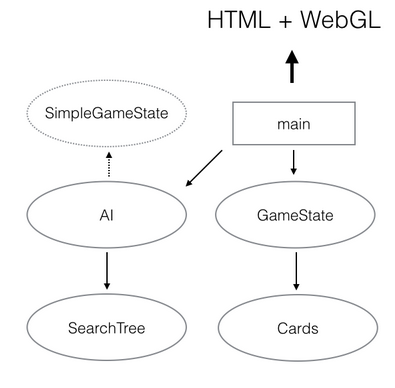
\includegraphics[scale=0.50]{img/arcitect.png}
    \caption{\label{fig:arcitect} A brief overview of the application architecture.}
  \end{center}
\end{figure}

\subsubsection{Game}
The main.js file is first painting the poker table and all buttons on the page, when the start button is clicked a GameState object and an AI object will be created.
The poker game is originated from the GameState object which only consists of a Cards object and functions for every state of the poker game. The game is created for two players where one player is an AI agent and the other player is the human player. The Cards object consist of a full deck of cards and all methods needed for playing Texas Hold'em like shuffle the deck of cards, deliver the flop, turn card, river card and cards for the players.

\subsubsection{AI}
The AI-file contains all methods necessary for the AI to be able to make a decision about what move to make. The heart of the AI is the method: findBestMove() which initializes a new instance of the SearchTree class and then runs the whole MCTS algorithm. The AI-file also contains methods for Hand Strength, Hand Potential and Effective Hand Strength. Bucketing, which has been mentioned earlier is also present and is used as a heuristic in the first round before the flop has been presented on the table.

\section{Result}
\subsection{The Game}
The result of this study is a Texas Hold'em game with an AI implemented using several different AI techniques combined together. The AI in the interactive game is using Monte Carlo Tree Search together with Hand Strength as a heuristic. The game is fully playable with an opponent that is realistic in the way it chooses which move to make. The 3D-scene is used to visualize the poker table, and it also shows the cards on hand. This is shown in Fig.\ref{fig:3dscene}.
\begin{figure}[H]
  \begin{center}
    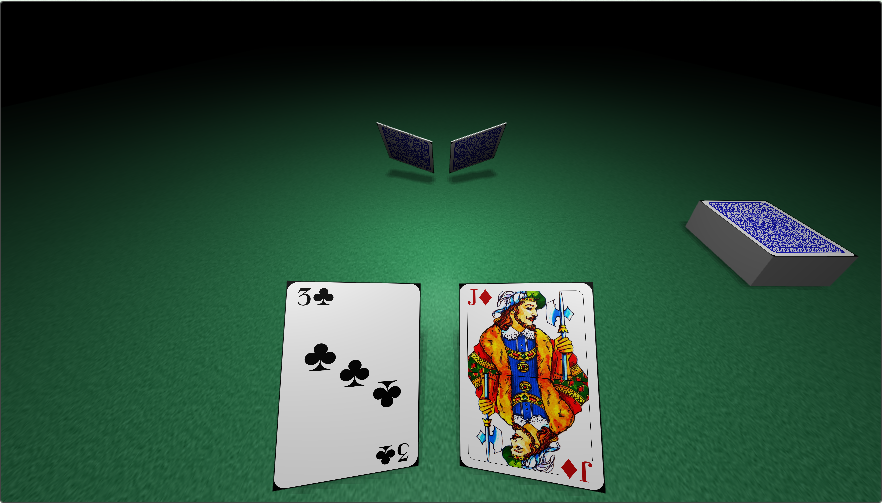
\includegraphics[scale=0.27]{img/3dscene.png}
    \caption{\label{fig:3dscene} The 3D-scene in the final version showing the player's cards on hand.}
  \end{center}
\end{figure}

To the left of the 3D-scene there are some additional UI-elements. these are the buttons telling the player what moves he or she can make. By pressing one of these buttons the player will make a move. The coloured buttons indicate that a move is valid. The greyed out buttons indicate invalid moves. The buttons are shown in Fig.\ref{fig:ui1}.
\begin{figure}[H]
  \begin{center}
    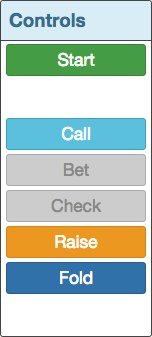
\includegraphics[scale=0.50]{img/ui1.png}
    \caption{\label{fig:ui1} The player controls, placed to the left of the 3D-scene. Greyed out buttons indicate an invalid move at the current state.}
  \end{center}
\end{figure}

To the right of the 3D-scene some information is shown. Information about money is visible in the upper box. How much money each player has, and how much money there is currently on the table. This information box is illustrated in Fig.\ref{fig:ui2}.
\begin{figure}[H]
  \begin{center}
    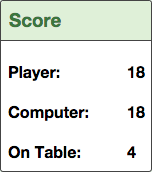
\includegraphics[scale=0.50]{img/ui2.png}
    \caption{\label{fig:ui2} The score board giving the player information about the money currently in play.}
  \end{center}
\end{figure}

Right below the score board, the enemy log is placed. It keeps track of what the AI does each time it makes a move. Since this is quite hard to visualize the decision was made to print the AI's move in text every time it makes a move. The enemy log is shown in fig(\ref{fig:ui3}).
\begin{figure}[H]
  \begin{center}
    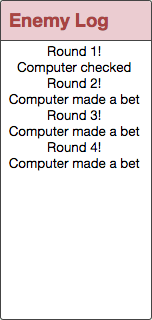
\includegraphics[scale=0.50]{img/ui4.png}
    \caption{\label{fig:ui3} The enemy log, showing what the AI has done each round.}
  \end{center}
\end{figure}

\subsection{Test results}
Since a number of algorithms were implemented in this study several results were achieved and therefore comparisons between the different approaches can be made. During this study, the different AI were put against each other playing several games. There are two different kinds of diagrams, one shows the percentage of won games and one shows the percentage of won hands. The following setups were made: 
\begin{itemize}
\item \textit{Monte Carlo + Hand Strength} vs \textit{Random Agent}
\item \textit{Effective Hand Strength} vs \textit{Monte Carlo + Hand Strength}
\item \textit{Monte Carlo} vs \textit{Monte Carlo + Hand Strength}
\item \textit{Monte Carlo + Hand Strength} vs \textit{Human Player}
\end{itemize}

\begin{figure}[H]
  \begin{center}
    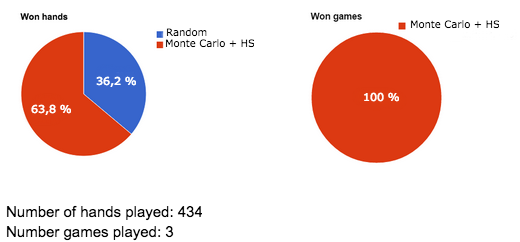
\includegraphics[scale=0.5]{img/randomvsmontehs2.png}
    \caption{\label{fig:randomvsmontehs} Result from Random vs Monte Carlo + Hand Strength.}
  \end{center}
\end{figure}

\begin{figure}[H]
  \begin{center}
    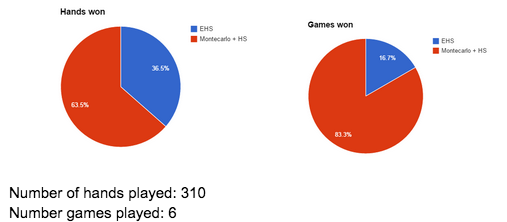
\includegraphics[scale=0.60]{img/montehsvsehs.png}
    \caption{\label{fig:montehsvsehs} Result from Monte Carlo + Hand Strength vs EHS.}
  \end{center}
\end{figure}

\begin{figure}[H]
  \begin{center}
    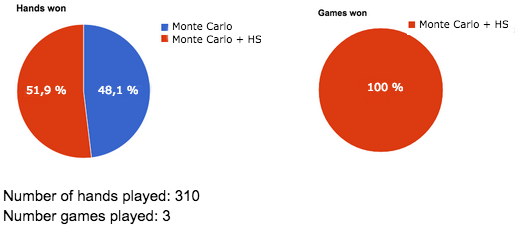
\includegraphics[scale=0.55]{img/montevsmontehsfixed.png}
    \caption{\label{fig:montevsmontehsfixed} Result from Monte Carlo vs Monte Carlo + HS (fixed number of simulations).}
  \end{center}
\end{figure}

\begin{figure}[H]
  \begin{center}
    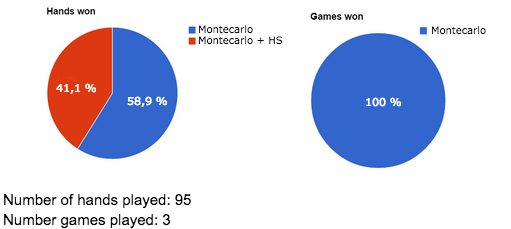
\includegraphics[scale=0.57]{img/montevsmontehs5sec.png}
    \caption{\label{fig:montevsmontehs5sec} Result from Monte Carlo vs Monte Carlo + HS (5sec time limit).}
  \end{center}
\end{figure}

\begin{figure}[H]
  \begin{center}
    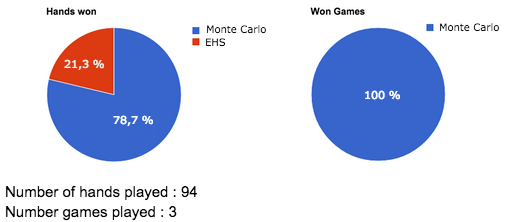
\includegraphics[scale=0.51]{img/montevsehs5sec.png}
    \caption{\label{fig:montevsehs5sec} Result from Monte Carlo vs EHS (5sec time limit).}
  \end{center}
\end{figure}

\subsubsection{\textit{Monte Carlo + Hand Strength} vs \textit{Human Player}}
When humans played against the AI it achieved about 45\% win rate over all games. All humans that played against it rated themselves as relative weak poker players and it would probably achieve worse result versus more experienced players. Three different persons participated in the tests against the AI. 

\section{Conclusion}
\subsection{Evaluation of the Result}
At a first glance it might look strange that the random agent won as many hands as it did, but one have to take into consideration that the amount of won hands is not the same as the amount of money won. The random agent wins a lot of hands, but this is due to the other agents often folding when they have bad cards. So the average size of the money pot is very small for the hands the random agent wins and much larger for the hands the other agents win. 

From the result it is clear that the Monte Carlo methods are stronger poker players than the rule based expert system that uses effective hand strength (EHS) to choose its moves. There could possibly be less difference between the agents if more time was spent refining the rules used by the EHS agent. 

Another interesting observation is that the Monte Carlo agent that uses Hand Strength to determine the moves in the simulation step loses to the one which does not, if both is constrained to 5 sec of simulations. The reason for this is that calculating the Hand Strength takes up a large portion of the simulation time, resulting in that the agent who does not use it can run 200 times more simulations. This shows that increasing the quality of the simulations is not always justified. 

On the other hand if we let both agents run a fixed amount of iterations, a 100\% win rate for the Monte Carlo agent that uses Hand Strength is achieved.

\subsection{Future Work}
\subsubsection{Opponent Modeling}
The quality of the solution given a certain number of iterations depends greatly on how good the simulation step can model the reality. For simple games it may be enough to simply use random moves, but for games as complicated as poker this will lead to a weak agent. The reason for this is that a player's actions is highly dependent on what cards he/she holds. Note that we are not interested in finding the most probable move of the opponent but the probability distribution over the available moves. The reason for this is that if we only get the most probable move then each simulation will result in the same sequence of actions. 

One simple approach is to model each opponent as a straight forward player, that means that we assume that an aggressive move (raise, bet) indicates a strong hand, and a passive move (check, call) indicates a weak hand. This can be implemented by holding a histogram with all stages (pre-flop, flop, turn, river) and all the actions taken by the player in those stages (fold, bet, call, raise, check). A raise in a game state indicates that a player has a strong hand if he usually does not raise in that state and vice versa. If the game goes to showdown it is possible to calculate the hand strength of the opponents cards on hand and thus making it possible to associate a hand strength with the actions taken that round\cite{schweizer}.

\subsubsection{Performance}
The quality of the MCTS solution depends on the amount of simulations it can make, the code in the project is far from optimized and it is probably easy to increase the number of simulations per round by refactoring and optimizing parts of the code. 

\subsubsection{Evaluation Against Human Player}
All evaluations have been performed between two poker agents in order to see which algorithm is winning but no exhaustive tests has been performed against human players. It would be interesting to see what results a skilled poker player would achieve against the AI.


\begin{thebibliography}{9}

\bibitem{Koller}
Daphne Koller and Avi Pfeffer. 1997. Representations and solutions for game-theoretic problems.Artif. Intell. 94, 1-2 (July 1997), 167-215. DOI=10.1016/S0004-3702(97)00023-4 

\bibitem{Metropolis}
Metropolis, N. (1987). The beginning of the Monte Carlo method. Los Alamos Science (1987 Special Issue dedicated to Stanislaw Ulam): 125�130.

\bibitem{levente}
Levente Kocsis and Csaba Szepesv�ri. 2006. Bandit based monte-carlo planning. In Proceedings of the 17th European conference on Machine Learning (ECML'06), Johannes F�rnkranz, Tobias Scheffer, and Myra Spiliopoulou (Eds.). Springer-Verlag, Berlin, Heidelberg, 282-293. DOI=10.1007/11871842\_29 
    
\bibitem{grze}
Grzegorz Fedczyszyn, Leszek Koszalka, and Iwona Pozniak-Koszalka. 2012. Opponent modeling in texas hold'em poker. In Proceedings of the 4th international conference on Computational Collective Intelligence: technologies and applications - Volume Part II (ICCCI'12), Ngoc-Thanh Nguyen, Kiem Hoang, and Piotr Jedrzejowicz (Eds.), Vol. Part II. Springer-Verlag, Berlin, Heidelberg, 182-191. DOI=10.1007/978-3-642-34707-8\_19

\bibitem{billingsburch}
 D. Billings, N. Burch, A. Davidson, R. Holte, J. Schaeffer, T. Schauenberg, and D. Szafron. 2003. Approximating game-theoretic optimal strategies for full-scale poker. In Proceedings of the 18th international joint conference on Artificial intelligence (IJCAI'03). Morgan Kaufmann Publishers Inc., San Francisco, CA, USA, 661-668.
 
\bibitem{billingspapp}
D. Billings, D. Papp, J. Schaeffer, and D. Szafron. Poker as a testbed for machine intelligence research. In Proceedings of Advances in Artificial Intelligence Research, pages 1-15, 1998b.

\bibitem{Chaslot} 
G.M.J.B. Chaslot, M.H.M. Winands, J.W.H.M. Uiterwijk, H.J. van den Herik, B. Bouzy (2008). Progressive Strategies for Monte-Carlo Tree Search. New Mathematics and Natural Computation 4 (3): 343�359.

\bibitem{papp}
Denis Richard Papp. 1998. Dealing with Imperfect Information in Poker. MS Thesis. University of Alberta, Edmonton, Alta., Canada. UML Order No. GAXMQ--34401.

\bibitem{davidson}
A. Davidson, D. Billings, J. Schaeffer, and D. Szafron. Improved opponent modeling in Poker. In Proceedings of the 2000 International Conference on Artificial Intelligence, pages 1467-1473, 2000.

\bibitem{broeck}
Guy Broeck, Kurt Driessens, and Jan Ramon. 2009. Monte-Carlo Tree Search in Poker Using Expected Reward Distributions. In Proceedings of the 1st Asian Conference on Machine Learning: Advances in Machine Learning (ACML '09), Zhi-Hua Zhou and Takashi Washio (Eds.). Springer-Verlag, Berlin, Heidelberg, 367-381. DOI=10.1007/978-3-642-05224-8\_28 

\bibitem{billingsdavidson}
Darse Billings, Aaron Davidson, Terence Schauenberg, Neil Burch, Michael Bowling, Robert Holte, Jonathan Schaeffer, and Duane Szafron. 2004. Game-Tree search with adaptation in stochastic imperfect-information games. In Proceedings of the 4th international conference on Computers and Games (CG'04), H. Jaap Herik, Yngvi Bj�rnsson, and Nathan S. Netanyahu (Eds.). Springer-Verlag, Berlin, Heidelberg, 21-34. DOI=10.1007/11674399\_2

\bibitem{schweizer}
Immanuel Schweizer, Kamill Panitzek, Sang-Hyeun Park, and Johannes F�rnkranz. 2009. An exploitative Monte-Carlo poker agent. In Proceedings of the 32nd annual German conference on Advances in artificial intelligence (KI'09), B�rbel Mertsching, Marcus Hund, and Zaheer Aziz (Eds.). Springer-Verlag, Berlin, Heidelberg, 65-72.

\bibitem{Kleij}
Van der Kleij, A. A. J.: Monte Carlo Tree Search and Opponent Modeling through Player Clustering in no-limit Texas Hold'em Poker. University of Groningen, The Netherlands (2010)

\bibitem{wenkai}
Wenkai Li and Lin Shang, "Estimating Winning Probability for Texas Hold'em Poker," International Journal of Machine Learning and Computing vol. 3, no. 1, pp. 70-74, 2013

\bibitem{pokerstars}
Rules for Texas Hold'em.(2014, October 31). Retrieved from http://www.pokerstars.se/poker/games/rules/ 

\bibitem{pokerlistings}
"Good Players vs. Winning Players in Poker" by Arthur Reber.(2011 January 6). Retrieved from http://www.pokerlistings.com/poker-strategy/good-players-vs-winning-players


\end{thebibliography}

\end{document}
